\section{Control Supervisado}
{\begin{small}%
\begin{flushright}%
\it
Entiende el problema y tendrás la solución
\end{flushright}%
\end{small}%
\vspace{.5cm}}
El presente proyecto de tesis consistió en un estudio y extensión del método previamente propuesto por Daniel Ciolek en su tesis de doctorado \cite{tesisDani}. Más precisamente, se trató de analizar carencias del algoritmo de exploración on-the-fly para problemas de Supervisory Control, cuya propiedad central era de tipo Non-blocking, y posteriormente analizados los problemas afrontarlos con una nueva especificación e implementación del algoritmo.

Un problema de Control Supervisado, dentro del área de AI Planning, consiste en un Sistema de Eventos Discreto (DES) con un subconjunto de sus estados marcados. Un factor clave de estos problemas es que el DES se presenta de forma modular tal que la composición paralela de múltiples componentes den lugar a la DES de interés. Desarrollaremos en mayor detalle las definiciones del problema en el capítulo~\ref{chpt:background}.

La motivación para analizar dichos problemas surge de la necesidad de verificar software, hoy en día utilizado en prácticamente todo emprendimiento humano. Si bien puede irse ganando confianza sobre la correctitud de un algoritmo a través de una bateria de tests, éstos no proveen una garantía si no una seguridad cada vez mayor. 

Un método alternativo es el de la verificación de la implementación del algoritmo con un modelo formal que cumpla los objetivos y requerimientos deseados del programa. Con esta visión en mente, el área de `Controller Synthesis` va un paso más allá y busca la generación automática de un controlador que dado un modelo (en forma de DES) cumpla siempre en toda ejecución posible los requisitos del problema.

Podemos trazar una comparación con el método de "Machine Learning", en auge desde hace unos años. En este paradigma, el programa tiene como input una multitud de casos de ejemplo del comportamiento buscado, si ponemos como ejemplo ganar un juego de ajedrez, tomaría una biblioteca de partidas jugadas de las cuales aprender. Como resultado, presentaría un programa que sabe jugar al ajedrez "muy bien", es decir, es muy probable que dada una partida, la gane, pero no está garantizado. Pueden verse hoy en día muchas aplicaciones de este método con gran éxito, desde la dominación del juego del "go" hasta autos manejados por IA. Sin embargo, ya que no ofrece ninguna garantía, es un método poco apropiado para sistemas críticos.

Como contraste, la Síntesis de controladores toma como input las reglas del juego de ajedrez, por ejemplo, varios componentes (autómatas) separados, siendo cada uno los movimientos posibles para una pieza. Como resultado, daría un controlador, que en cada momento de la partida solo habilita algunas de las transiciones de los autómatas y garantiza que si se le hace caso ganará la partida. Es esencial notar que la técnica de este trabajo busca obtener una garantía muy fuerte, y el problema lo encuentra en la escalabilidad del problema, ya que hoy en día es imposible aplicarla a un juego del tamaño del ajedrez.

\section{Caso de estudio}
A continuación se presenta un ejemplo sobre el cual aplicaremos nuestro algoritmo a lo largo de la presentación. 

Imaginemos un negocio del cual modelamos 3 componentes: La cuenta de dinero, la estación de ventas de productos terminados, y la estación de compra de materia prima y ensamblaje de productos.

La cuenta de dinero puede estar vacía o con dinero, no contamos cuanto dinero hay, pero sabemos que en caso de estar vacía no se pueden comprar nuevas materias primas. También podemos elegir al momento de comprar nuevos materiales si queremos gastar todo el dinero que hay en la cuenta o solo gasta una parte.

La estación de ensamble puede necesitar comprar nuevos materiales, y una vez que los recibe necesita un tiempo no controlable hasta finalizar el próximo producto, momento en el que el mismo se transfiere a la estación de ventas.

La estación de ventas, cuando tiene un producto para vender, tarda un tiempo no controlable hasta que llega un cliente que compra el producto, momento en el que la cuenta del negocio guarda la plata y seguramente no está vacía.

Mostramos en la figura~\ref{fig:modelos} un LTS (Labeled transition system) para cada uno de los componentes descriptos.


\begin{figure}[htb]
	\begin{center}
	\makebox[\linewidth][c]{%
	\begin{subfigure}[t]{.7\textwidth}
		\centering
		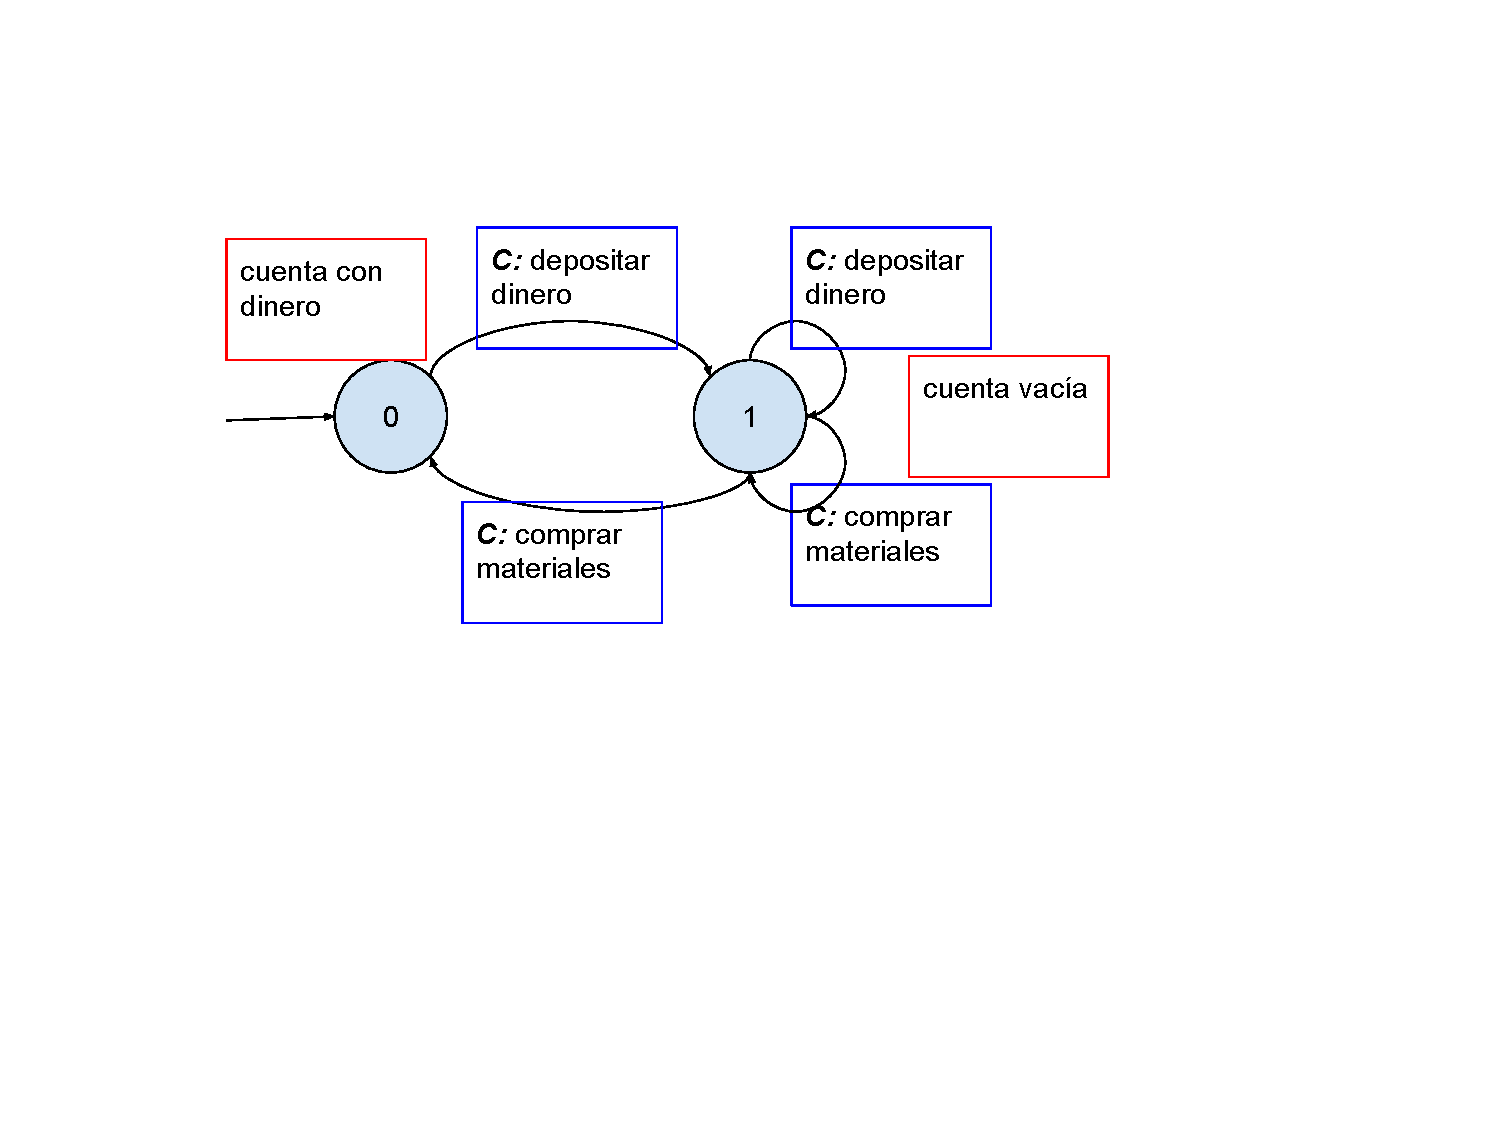
\includegraphics[width=\linewidth]{figures/ModeloCuentaBanco.pdf}  
		\caption{Cuenta bancaria}
		\label{fig:ModeloBanco}
	\end{subfigure}
	\begin{subfigure}[t]{.7\textwidth}
		\centering
		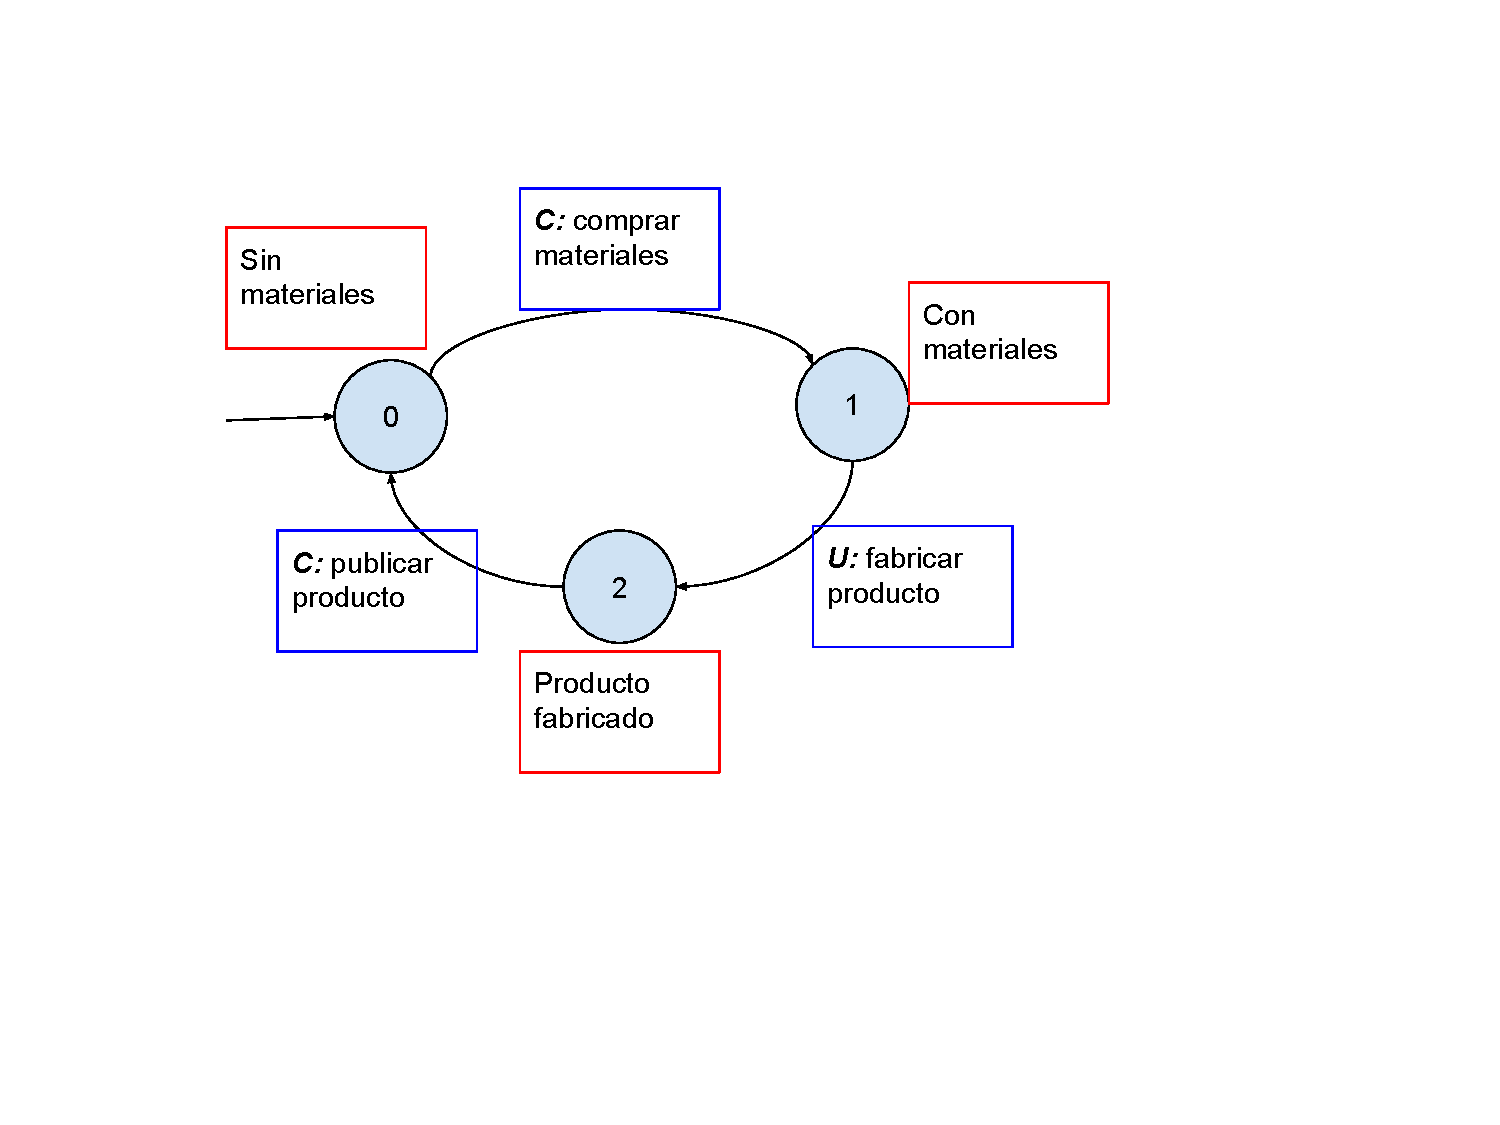
\includegraphics[width=\linewidth]{figures/ModeloEnsamblaje.pdf}  
		\caption{Estacion de ensamblaje}
		\label{fig:modeloEnsamblajes}
	\end{subfigure}
	}
	\makebox[\linewidth][c]{%
	\begin{subfigure}[t]{.7\textwidth}
		\centering
		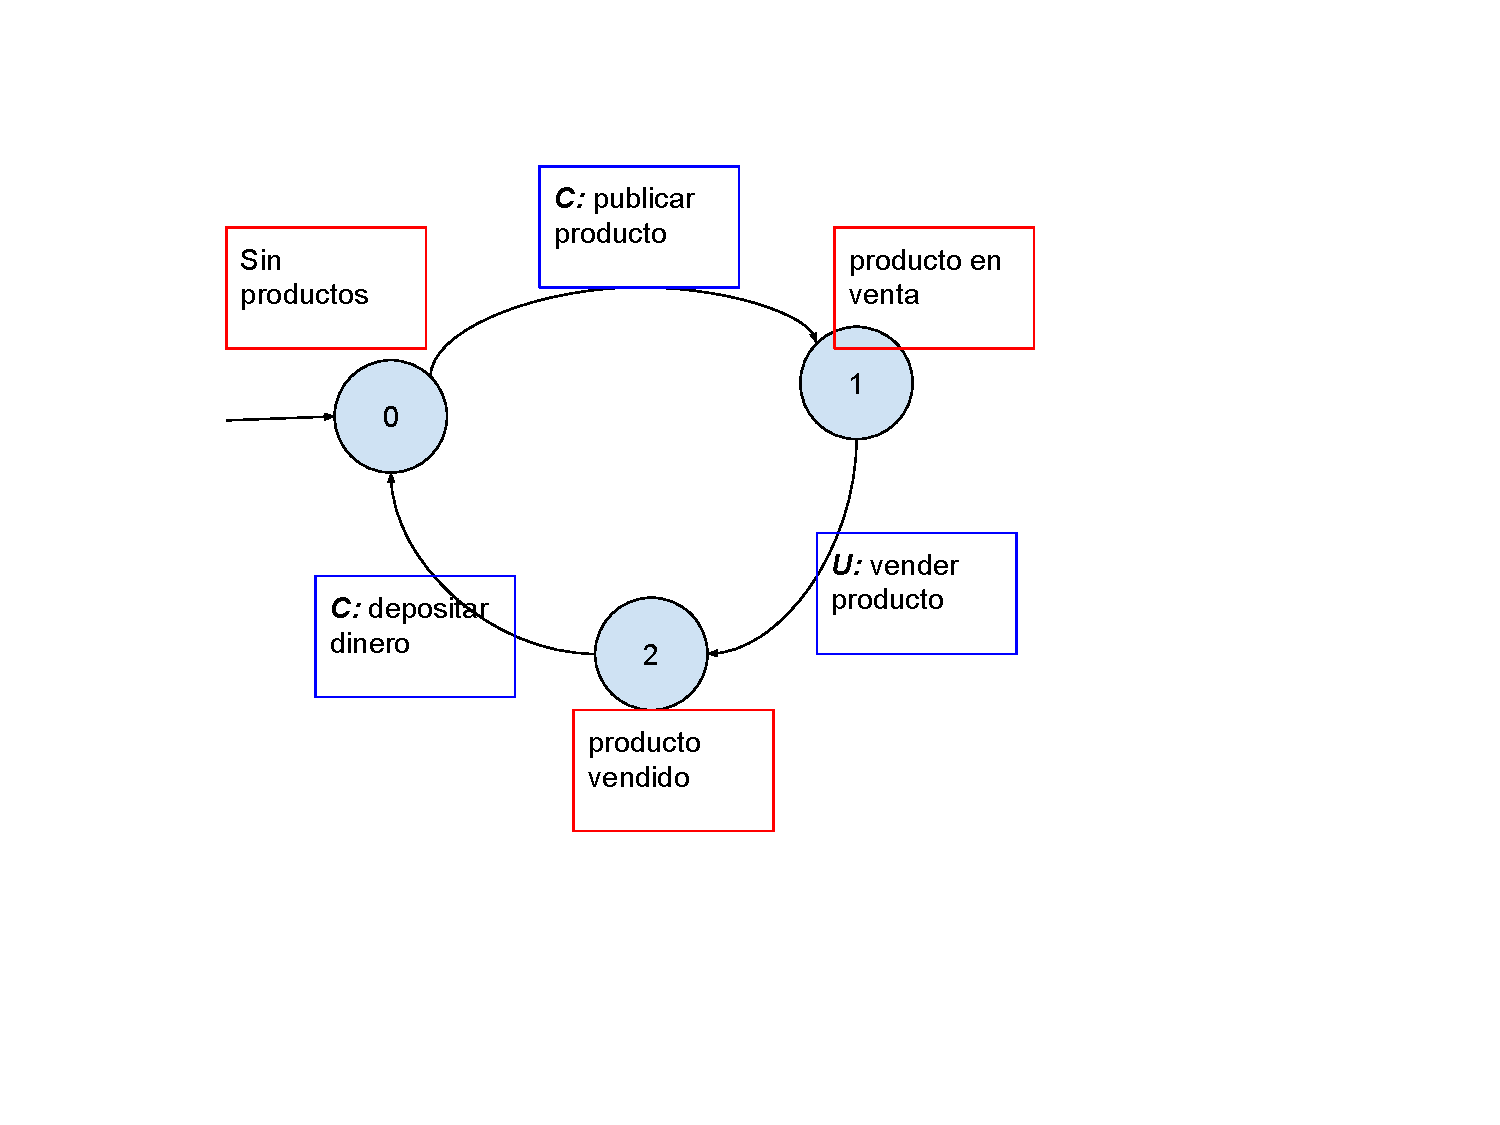
\includegraphics[width=\linewidth]{figures/ModeloVentas.pdf}  
		\caption{Estacion de ventas}
		\label{fig:modeloVentas}
	\end{subfigure}
	\begin{subfigure}[t]{.7\textwidth}
	\centering
	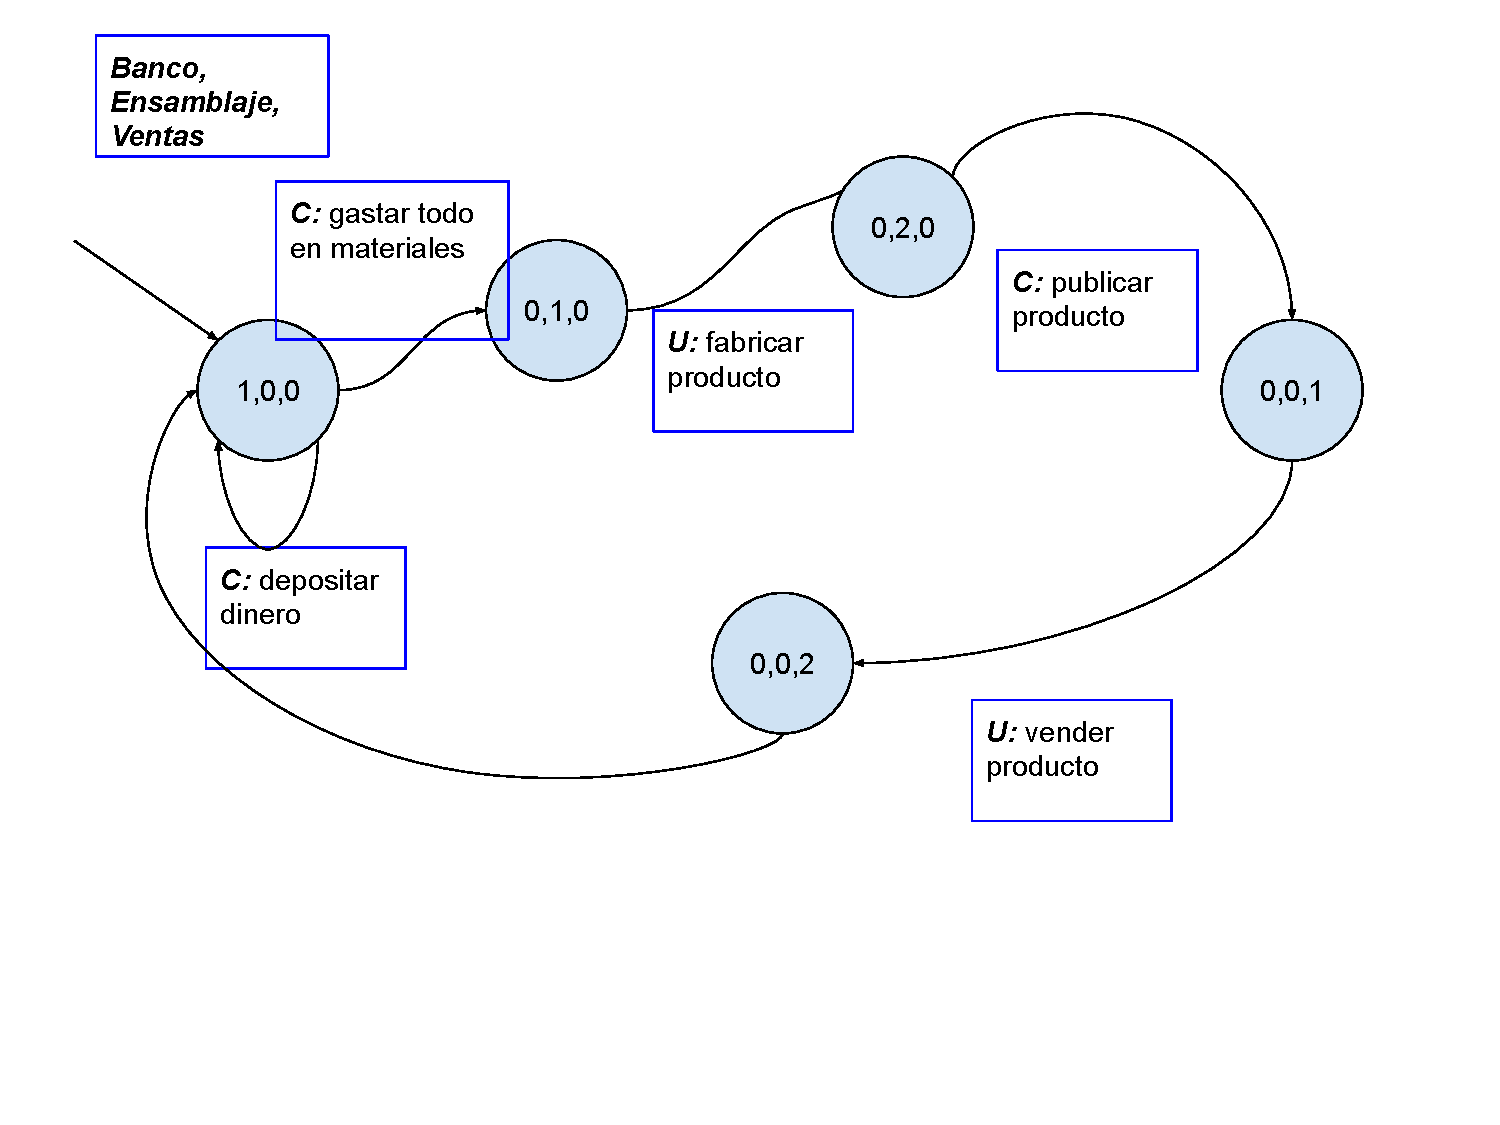
\includegraphics[width=\linewidth]{figures/ModeloCompuestoSin2Caminos.pdf}  
	\caption{Composición de los componentes}
	\label{fig:compuesto}
	\end{subfigure}
	}
	\caption{Modelo de ejemplo}
	\label{fig:modelos}
	\end{center}
\end{figure}




















